
\section{Data preparation and periodogram calculation}

All the classical Cepheid data from the OGLE download site was downloaded using an script (\autoref{lst:download})
designed to replicate the folder tree of the site, for better programatic access to the data.
The downloaded files amount to $\sim$47 MB.

Next, the pandas library \citep{pandas} was used to perform the statistical analysis shown on \autoref{sec:data}.
Accordingly to the stated there, only the $I$ magnitude data was used to search for the period.

Following the sample benchmark done on \autoref{fig:runtimes}, 
the incremental implementation of the Fourier periodogram (\autoref{lst:fourier})) was selected to find the period of each star with $I$ magnitude data.
A linear frequency grid was used to calculate the periodogram, starting from $\nu_0=0.001$/day ($P= 1000$ days), 
incrementing on steps of $d\nu = 10^{-5}$/day, up to $\nu_f=4.7$/day ($P=0.212$ days), giving a total of 469900 test frequencies, 
99000 of which are in the $(1,100)$ days period range.
With a modification on the implementation, an linear period grid could be used instead with the incremental transform.
The ideal grid would be linear on $\log P$, as that is the variable in which the PL relation is linear; 
however, the faster incremental implementation cannot be unsed on an uneven grid, and so the slower Lomb-Scargle or simple Fourier periodogram must be used instead.

As deduced in \autoref{sec:examples-and-aliases}, 
the magnitude data was normalized to zero mean to prevent finding false peaks caused by the near-periodic cadence of the data.
After that, each periodogram was calculated, and normalized to the principal (highest) peak.
A peak detection algorithm by SciPy \citep{scipy} was used to capture the secondary peaks which height were greater than half the principal peak.
This was motivated by the intuition that if a spectrum has many high peaks, 
the true frequency would be uncertain, and that could be later used as a criterion to clean the PL diagram from outliers.
The peak widths at half maximum were calculated, as this is the only measure of the uncertainty of the found frequency at our disposal.
This frequency uncertainties were never greater than 0.0014/day.

After every star on each Cloud have passed through this process, the results were saved in one structured data file, in this case in the \texttt{JSON} format.
The number of detected peaks on the spectrum, compared to the number of data points available for each star, can be found in \autoref{fig:peaks-n-points}.
Limits to the number of detected peaks and data points were decided to eliminate outliers from the next step, which is the PL relation, the main result.

\begin{figure}
	\centering
	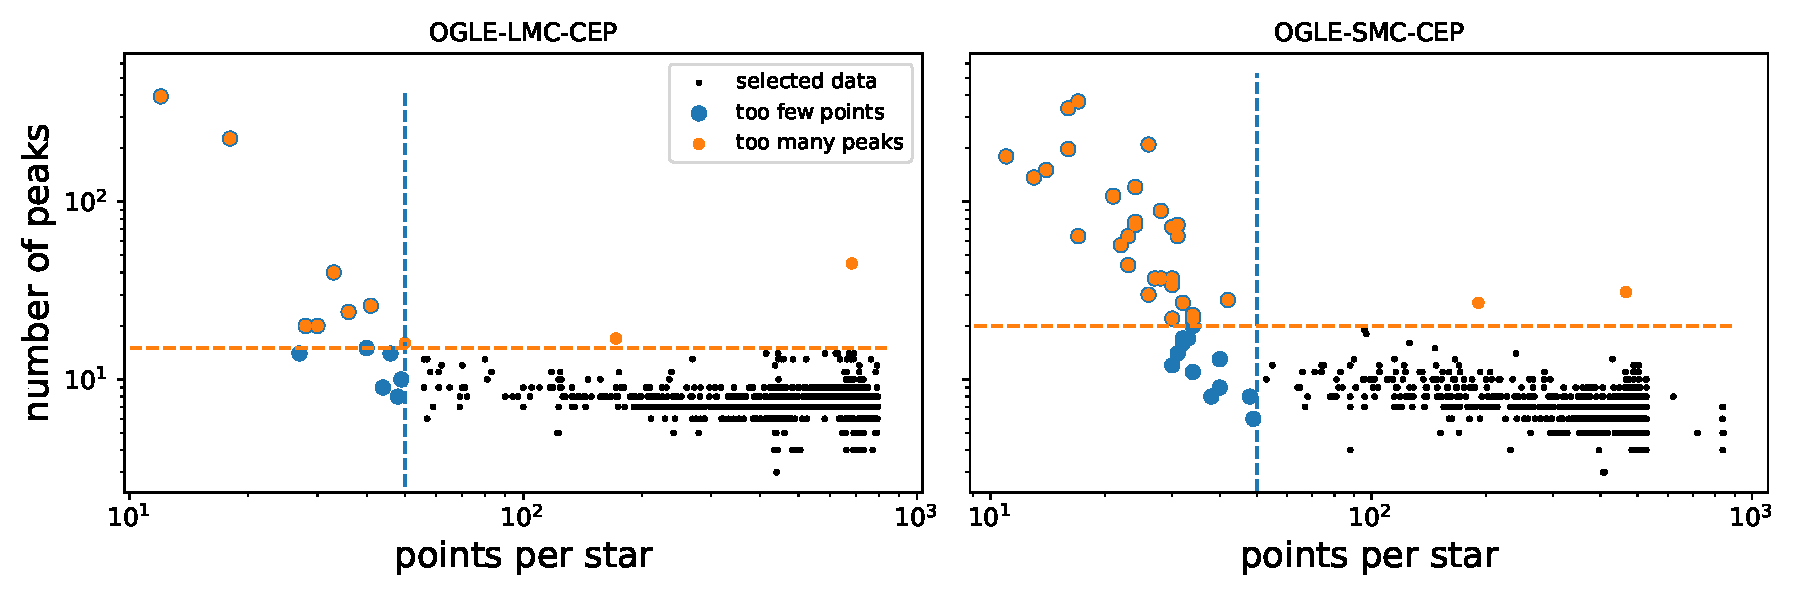
\includegraphics[width=0.9\textwidth]{img/peaks_vs_points.pdf}
	\caption[Results: detected number of peaks against data size]{
		Detected number of peaks plotted against the size of the data for each Cepheid in the Magellanic Clouds.
		The stars with less than 50 points were considered to have too little data to conclude that the frequency found with the algorithm is indeed the correct one.
		The same doubt is casted on those stars with a high number of peaks in the spectrum. The limit is 15 peaks for the LMC and 20 for the SMC.
		Those limits were chosen to maximize the number of outliers discarded from the PL relation (\autoref{fig:pl-result}) whithout discarding seemingly good placed stars in the PL diagram.
	}
	\label{fig:peaks-n-points}
\end{figure}


\autoref{eq:wesenheit-i} was used to calculate the extinction-free Wesenheit index, 
with $R_I=1.55$ \citep{OGLE2015,Ulaczyk2013} and the mean $I$ and $V$ mangitude for each star.
Uncertainty in the mean of each magnitude was also computed, using contribution from two factors.
The first was compound uncertainty, using the errors reported for each magnitude measurement, calculated as $1/\sigma_{total}=\sqrt{\sum_i 1/\sigma_i^2}$.
The second factor was estimated via bootstrap, as the standard deviation of the mean from several resamplings of the magnitudes.
The resulting uncertainties were never greater than 0.04 mag, for the selected data. 
The distribution of uncertainties is plotted on \autoref{fig:uncertainties}, 
and its corresponding error bars on the PL diagram would be barely even visible.

\begin{figure}
	\centering
	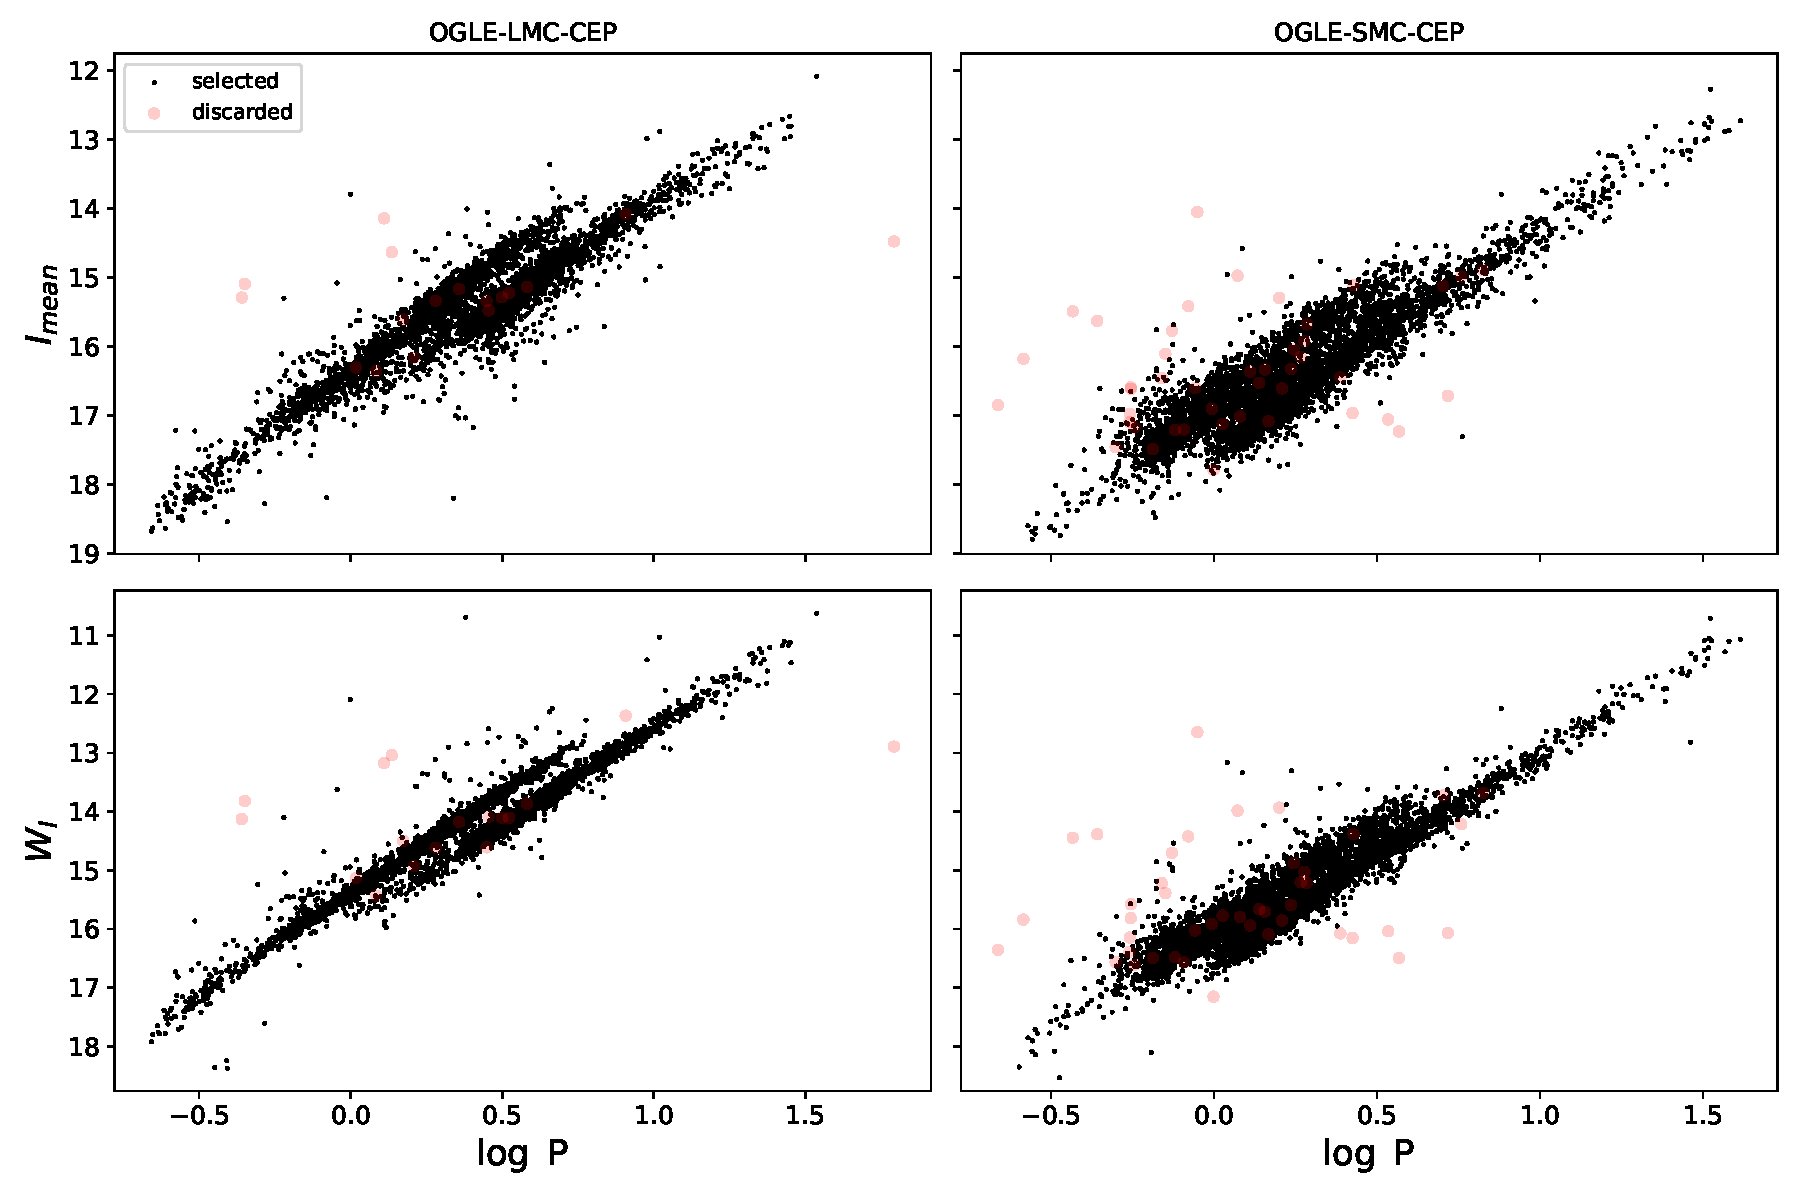
\includegraphics[width=\textwidth]{img/PL_realtion.pdf}
	\caption[Results: PL relation for the Magellanic Clouds]{
		Period-Luminosity diagrams for classical Cepheids int he Magellanic Clouds, on $I$ magnitude and $W_I$ index.
		Discarded stars accoring to the criteria presented in \autoref{fig:peaks-n-points} are shown as faint red shadows.
		In each diagram, two main linear tendencies can be noted, the fundamental and the first overtone tendencies.
		It is notable how well the Wesenheit index separates the two tendencies, especially in the LMC.
	}
	\label{fig:pl-result}
\end{figure}

\section{PL relations for the Magellanic Clouds}

If we plot the Wesenheit index against the frequencies of the highest peak for each star, remembering that $\log P=-\log \nu$, we obtain \autoref{fig:pl-result},
the Period-Luminosity relation for the Magellanic Clouds. This is a good reproduction of the results from \cite{OGLE2016}, 
from where we can associate the lower linear tendency to the \texttt{F} pulsation mode and the upper one with the \texttt{1O} mode, or the first overtone.
Some few stars of the \texttt{2O} mode can be observed at the back of the \texttt{1O} tendency, around $\log P\approx 0$.
This is of course just a general association, given that we did not perform pulsation mode analysis on these results.
Also, multimode pulsators like \texttt{F1O} or \texttt{1O2O} cannot be separated from their lowest frequency on this kind of PL diagram.



The Wesenheit index is as sucessful as expected on reducing the dispersion on the diagram.
This method is just a mean approximation of the reddening, and as such, it is limited, but great separation is achieved on the LMC diagram.
The disperison, however, is far grater in the SMC compared to the LMC. 
Despite this specific dataset having fewer points per star in the SMC, this should not be an artifact of the data, 
but a result of the SMC being farther away than the LMC, at $62.44 \pm_{stat} 0.47 \pm_{sys}0.81$ kpc 
and $49.97 \pm_{stat} 0.19 \pm_{sys} 1.11$ kpc respectively \citep{SMC2020,LMC2013}.

\subsection{Comparison with OGLE-IV results}


Some disperse points in the PL diagram were also present in the OGLE results. 
Those stars could be just missclassified, something that occurs fairly often \citep[see for example Table 1 of][]{OGLE2016};
some stars previously thought to be classical Cepheids turned out to be of the RR Lyr\ae{} class,
or anomalous Cepheids, or even Eclipsing variables.

Our results, however, are not in perfect agreement with those of \cite{OGLE2016}.
Several outliers can be seen in the diagrams presented here, but some of those are also in the OGLE-IV results.
Fortunately, in the download site there are several \texttt{*.cep} files that contain the periods found by them.
Using that data, we can directly compare the results, information presented in \autoref{fig:comparison}.

\begin{figure}
	\centering
	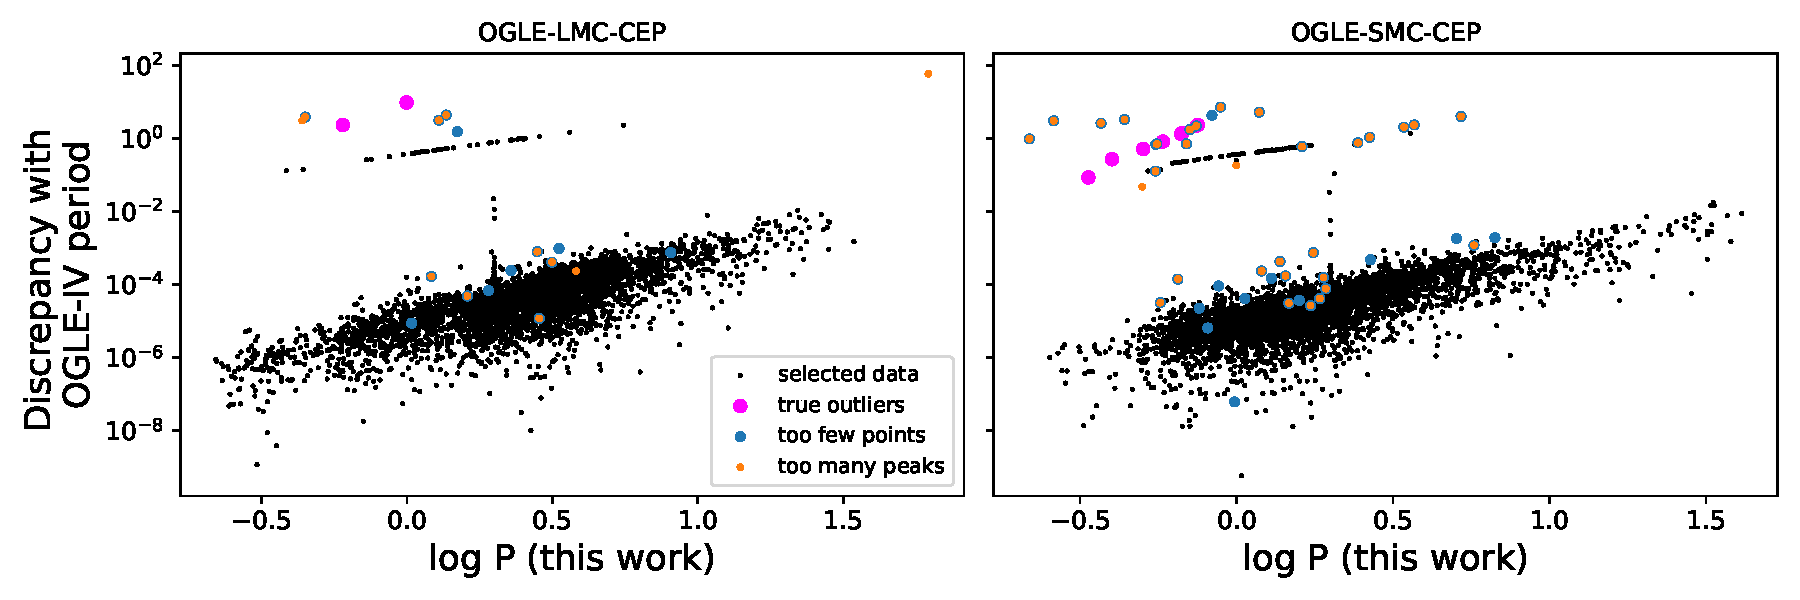
\includegraphics[width=0.95\textwidth]{img/discrepancies.pdf}
	\caption[Results: comparison with OGLE-IV periods]{
		Absolute differences between the periods found on this work and those found on the OGLE data site, as a function of $\log P$.
		Five groups can be discerned: (1): the bulk of stars, those in accordance to the OGLE period, shown in black. 
		(2): a tiny subset of those, forming a near vertical line of increasing discrepancy, at around  $\log P = 0.3$, and connects with
		(3): a thin horizontal line of stars with discrepancy of about 0.1 to 1.
		(3) and (4): the points excluded from the PL relation since \autoref{fig:peaks-n-points}, on blue and orange.
		(5): the remaining points with high error after removing (2-4), denominated \enquote{true outliers}, shown in magenta.
	}
	\label{fig:comparison}
\end{figure}

The majority of stars are located in the low discrepancy side of that diagram, which means there are general agreement with the OGLE results;
98\% of the stars with both $I$ and $V$ data were found in this work to have a period that did not differ from the OGLE period more than $0.01$ days.
In the LMC there were 51 stars with a discrepancy greater than 0.01 days, and 84 in the SMC.

A general trend can be observed: the discrepancy is larger the larger the period.
This suggest that a period grid, not a frequency one, was used to produce th OGLE results.

\begin{figure}
	\centering
	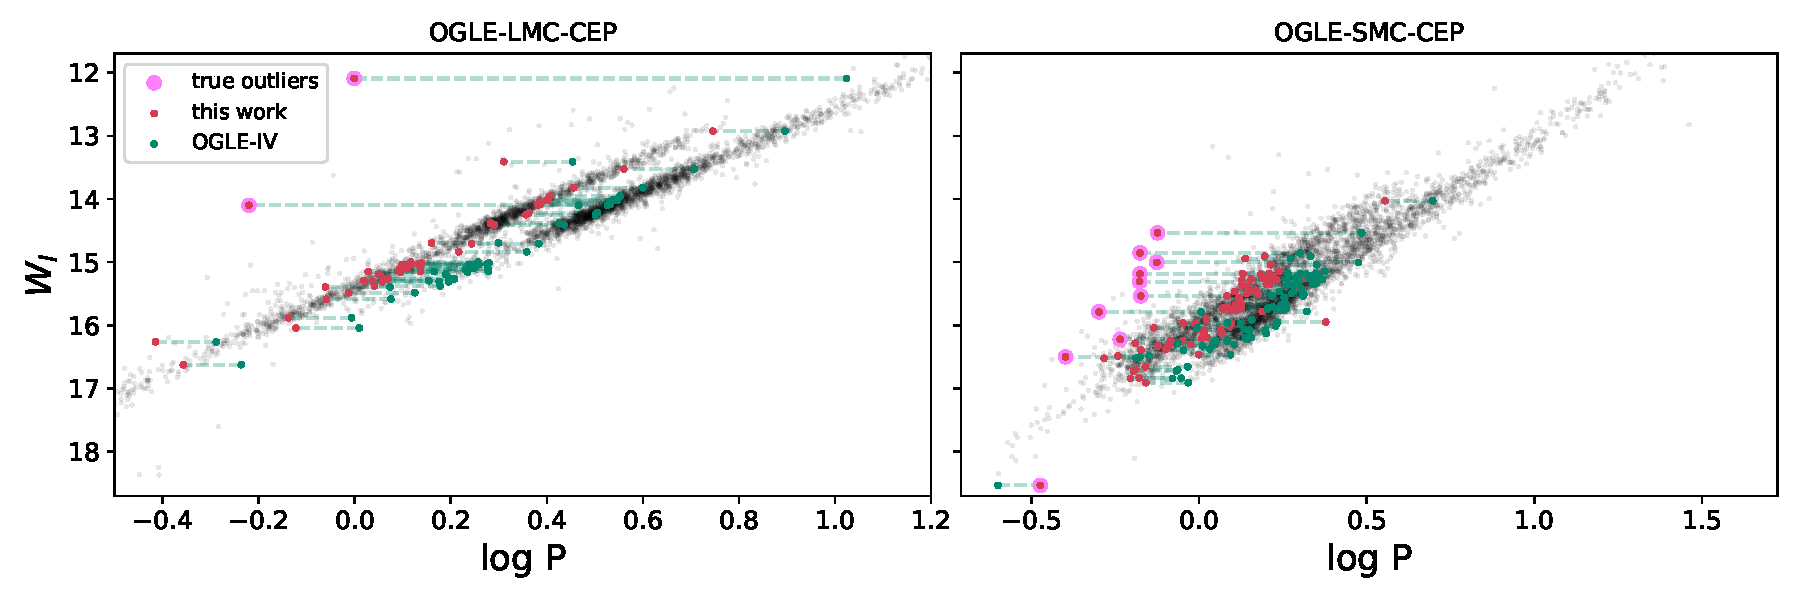
\includegraphics[width=\textwidth]{img/horizontal_line_corrections.pdf}
	\caption[Results: comparison with OGLE-IV periods]{
		Differences on period for the horizontal line (3) from \autoref{fig:comparison} and true outliers (5), when using the period found in this work (on red)
		and the displacement  (green dashed line) to their positions when using the periods from OGLE (on green).
		Big magenta circles are drawn on the true outliers from  \autoref{fig:comparison}.
	}
	\label{fig:horizontal-line-corrections}
\end{figure}

\subsubsection{The horizontal line}

But there is a more intresting feature in that graphic: a very thin line of stars with discrepancy larger than 0.02, 
too well organized to be the result of few data points or poor random sampling.
The effect is clearly systematic, yet no a priori way of isolating this line from the data was found.
Manually selecting this region in \autoref{fig:comparison}, 
we could track their $\log P$ movement in the PL diagram if we use our periods and OGLE's.
That is plotted in \autoref{fig:horizontal-line-corrections}.
Almost all of those stars are in the \texttt{1O} tendency when using the periods found on this work,
and pass to the \texttt{F} tendency when using the periods from OGLE. 

With that information one could suspect that these were multimode \texttt{F1O} Cepheids 
that our algorithm just happened to found by their first overtone frequency rather than their fundamental one.
A reverse search in the OGLE classification files for the code of these stars confirms that, indeed, 
of the 45 stars on the horizontal discrepancy line of the LMC, 44 of them were classified as \texttt{F1O} pulsators.
The remaining star, code \texttt{1378}, was a \texttt{F1O2O} multimode, so in fact the argument holds.
For the SMC case, there were 69 stars on the line, with 63 of them being \texttt{F1O} pulsators.
Here the correlation ends, as the remaining six were four fundamental (\texttt{0473},\texttt{1029},\texttt{2792},\texttt{4675}) 
and two \texttt{1O2O} ones (\texttt{0998}, \texttt{4784}).
By better analyzing the overtone content of these stars, 
their pulsation modes could be taken into account to place them in the proper side of the PL tendencies,
eliminating the systematic line of \autoref{fig:comparison}.

\subsubsection{The vertical line}

The next thing that jumps into view from \autoref{fig:comparison} is the tiny bridge 
that connects the low error results with the horizontal line (2).
A detailed plot of those points can be seen in \autoref{fig:vertical-discrepancy}. 
On the selected range, which is somewhat arbitrary on the low error side, there are 13 stars for the LMC and 12 on the SMC.
Most of those stars are \texttt{1O} pulsators for the LMC and \texttt{F} pulsators for the SMC, 
and they are placed in between of the two tendencies of the PL diagram, so the missclasification argument presented above does not hold.
Like before, no a priori way of detecting these stars was found.

\subsubsection{The true outliers}

The magenta dots on \autoref{fig:horizontal-line-corrections} represent the true outliers, 
those few for which the period found in this work differ significantly from the OGLE period,
despite having a typical number of data points and also a typical number of peaks in their spectrum.
This could mean that the algorithm simply failed, either because some irregularity on the data or in the implementation. 

The two outliers of the LMC have OGLE codes \texttt{0016} and \texttt{4668}, and are fundamental pulsators according to OGLE.
The 10 SMC ones have codes 
\texttt{1400}, 
\texttt{2521}, 
\texttt{2924}, 
\texttt{3108}, 
\texttt{4020}, 
\texttt{4361}, and
\texttt{4967} (fundamental pulsators);
\texttt{3317} and
\texttt{4195} (\texttt{1O} pulsators); and 
\texttt{1350} (\texttt{1O2O} pulsator).

% lastly, the true outsiders

\subsection{Secondary peaks in the PL diagram}

A diminished reflection of the spectrum near integer frequencies was found for nearly all individual stars,
as the blue spectrum illustrated in \autoref{fig:uneven-advantage}.
That resulted on the secondary peaks of each star spectrum to form patterns around those points of integer frequencies.

Some of the frequencies found for some stars lied on that secondary peak zone, indicating that they were not the optimal period for that star.
This can possibly be solved by refining the search around all the peaks found above the noise of the spectrum.
As can be seen in \autoref{fig:peaks-n-points}, the number of peaks is of the order of $\sim20$ or less for stars with a reasonable amount of data,
so this aditional search with a finer grid, perhaps in the interval $[\nu_{peak}-\,d\nu,\nu_{peak}+\,d\nu]$, should not take too much of additional processor time,
and can be performed using any of the algorithms discussed in this work, as false peaks have been eliminated in the first run.

A PL diagram on linear frequency of these secondary peaks, demonstrating the analogy with \autoref{fig:uneven-advantage}, is presented on \autoref{fig:linear-color-pl-lmc}.
Versions of \autoref{fig:pl-result} with those same secondary peaks for both Clouds are in \autoref{fig:color-pl-lmc} and \autoref{fig:color-pl-smc},
where the missplaced principal peaks of the outliers can be seen lying with the secondary peaks.


% additional peaks diagrams on the appendix
% those true outliers are positioned in the second peak of the spectrum in the colorful figures
%some yellow dots can be seen lying around the secondary peaks. This can possibly be resolved by searching with a fined $d\tau$ around each founded peak, 
% to find the true maximum of each one. This can be done with any of the five algorithms, as the speed should not be a problem for so few points.